\documentclass[a4paper,10pt]{article}
\usepackage[dvips]{color,graphicx}
\usepackage[dvips, bookmarks, colorlinks=false]{hyperref}


%opening
\title{Math650 Homework 8}
\author{Yu Huang}
\date{2006-10-19}

\begin{document}

\maketitle


\section{Question 1}
The four different contrast functions result differrent contrast matricies. Details see page 146 Book by Venables et al, 2002.

However, if we only look at the identifiability contraint, \emph{contr.helmert}, \emph{contr.sum} and \emph{contr.poly} are same, which is $1^T\alpha=0$ (the sum of coefficients equals to zero). \emph{contr.treatment}, which is the default option in R, sets the first coefficient to 0 and the rest of them correspond to level 1.

\begin{verbatim}
> options(contrasts=c("contr.sum", "contr.sum"))
> test_contr2()
  [,1] [,2]
0    1    0
1    0    1
2   -1   -1
> options(contrasts = c("contr.treatment", "contr.poly"))
> test_contr2()
  1 2
0 0 0
1 1 0
2 0 1
> options(contrasts = c("contr.helmert", "contr.poly"))
> test_contr2()
  [,1] [,2]
0   -1   -1
1    1   -1
2    0    2
> options(contrasts = c("contr.poly", "contr.poly"))
> test_contr2()
             .L         .Q
0 -7.071068e-01  0.4082483
1 -9.073264e-17 -0.8164966
2  7.071068e-01  0.4082483
\end{verbatim}


\section{Question 2}
Based on the analysis of the identifiability contraint above, different contrasts play between \emph{intercept} and factor-involved coefficients. Contrasts with same identifiability contraint gave similar(almost identical, but due to float differences) results.

\subsection{contr.treatment}
This is the default.
\begin{verbatim}
Call:
lm(formula = LOGIT ~ LOGDURATION + BEE + LOGDURATION * BEE, data = data)

Residuals:
    Min      1Q  Median      3Q     Max
-1.3804 -0.3699  0.0307  0.4552  1.1611

Coefficients:
                      Estimate Std. Error t value Pr(>|t|)
(Intercept)            -3.0390     0.5115  -5.941 4.45e-07 ***
LOGDURATION             1.0121     0.1902   5.321 3.52e-06 ***
BEEWORKER               1.3770     0.8722   1.579    0.122
LOGDURATION:BEEWORKER  -0.2709     0.2817  -0.962    0.342
---
Signif. codes:  0 '***' 0.001 '**' 0.01 '*' 0.05 '.' 0.1 ' ' 1

Residual standard error: 0.6525 on 43 degrees of freedom
Multiple R-Squared: 0.6151,     Adjusted R-squared: 0.5882
F-statistic:  22.9 on 3 and 43 DF,  p-value: 5.151e-09
\end{verbatim}

\subsection{contr.helmert}
\begin{verbatim}
Call:
lm(formula = LOGIT ~ LOGDURATION + BEE + LOGDURATION * BEE, data = data)

Residuals:
    Min      1Q  Median      3Q     Max
-1.3804 -0.3699  0.0307  0.4552  1.1611

Coefficients:
                 Estimate Std. Error t value Pr(>|t|)
(Intercept)       -2.3505     0.4361  -5.390 2.80e-06 ***
LOGDURATION        0.8766     0.1408   6.224 1.72e-07 ***
BEE1               0.6885     0.4361   1.579    0.122
LOGDURATION:BEE1  -0.1354     0.1408  -0.962    0.342
---
Signif. codes:  0 '***' 0.001 '**' 0.01 '*' 0.05 '.' 0.1 ' ' 1

Residual standard error: 0.6525 on 43 degrees of freedom
Multiple R-Squared: 0.6151,     Adjusted R-squared: 0.5882
F-statistic:  22.9 on 3 and 43 DF,  p-value: 5.151e-09
\end{verbatim}

\subsection{contr.sum}
\begin{verbatim}
Call:
lm(formula = LOGIT ~ LOGDURATION + BEE + LOGDURATION * BEE, data = data)

Residuals:
    Min      1Q  Median      3Q     Max
-1.3804 -0.3699  0.0307  0.4552  1.1611

Coefficients:
                 Estimate Std. Error t value Pr(>|t|)
(Intercept)       -2.3505     0.4361  -5.390 2.80e-06 ***
LOGDURATION        0.8766     0.1408   6.224 1.72e-07 ***
BEE1              -0.6885     0.4361  -1.579    0.122
LOGDURATION:BEE1   0.1354     0.1408   0.962    0.342
---
Signif. codes:  0 '***' 0.001 '**' 0.01 '*' 0.05 '.' 0.1 ' ' 1

Residual standard error: 0.6525 on 43 degrees of freedom
Multiple R-Squared: 0.6151,     Adjusted R-squared: 0.5882
F-statistic:  22.9 on 3 and 43 DF,  p-value: 5.151e-09
\end{verbatim}

\subsection{contr.poly}
\begin{verbatim}
Call:
lm(formula = LOGIT ~ LOGDURATION + BEE + LOGDURATION * BEE, data = data)

Residuals:
    Min      1Q  Median      3Q     Max
-1.3804 -0.3699  0.0307  0.4552  1.1611

Coefficients:
                  Estimate Std. Error t value Pr(>|t|)
(Intercept)        -2.3505     0.4361  -5.390 2.80e-06 ***
LOGDURATION         0.8766     0.1408   6.224 1.72e-07 ***
BEE.L               0.9737     0.6167   1.579    0.122
LOGDURATION:BEE.L  -0.1916     0.1992  -0.962    0.342
---
Signif. codes:  0 '***' 0.001 '**' 0.01 '*' 0.05 '.' 0.1 ' ' 1

Residual standard error: 0.6525 on 43 degrees of freedom
Multiple R-Squared: 0.6151,     Adjusted R-squared: 0.5882
F-statistic:  22.9 on 3 and 43 DF,  p-value: 5.151e-09
\end{verbatim}

Most differences happen to the \emph{intercept}, coefficients of \emph{BEE} and \emph{LOGDURATION:BEE}. \emph{contr.sum} and \emph{contr.helmert} yielded the identical results. \emph{contr.poly} doesn't fit in this scenario very well as it's catered towards ordered factor variables.

\section{Question 3}
I tried three different breakdown points and see how the regression line changes and residual plots et al.
\newline
\begin{tabular}{|r|r|r|r|r|}
\hline
data\_type & $\alpha$(breakdown point) & intercept & coeff LOGDURATION & scale estimates\\
\hline
queen & 0.9 & -3.039 & 1.012 & 0.6817 \\
\hline
worker & 0.9 & -1.6753 & 0.7129 & 0.4338 \\
\hline
queen & 0.8 & -2.9255 & 0.9844 & 0.734 \\
\hline
worker & 0.8 & -1.6753 & 0.7129 & 0.4464 \\
\hline
queen & 0.6 & -3.303 & 1.142 & 0.7505 \\
\hline
worker & 0.6 & -1.6753 & 0.7129 & 0.4504 \\
\hline
\end{tabular}


Figures~\ref{f2} and ~\ref{f3} are for $\alpha=0.9$. Figures~\ref{f4} and ~\ref{f5} are for $\alpha=0.8$. Figures~\ref{f6} and ~\ref{f7} are for $\alpha=0.6$. The WORKER's data is pretty robust while QUEEN's data shows quite fluctuation with the change of $\alpha$.

\begin{figure}
\includegraphics[angle=-90, width=1\textwidth]{figures/math650_hw8_fig1.eps}
\caption{Scatterplot of LOGIT vs LOGDURATION}\label{f1}
\end{figure}
\begin{figure}
\includegraphics[angle=-90, width=1\textwidth]{figures/math650_hw8_fig2_alpha0_9.eps}
\caption{Linear regression plots without interaction and full data, alpha=0.9}\label{f2}
\end{figure}
\begin{figure}
\includegraphics[angle=-90, width=1\textwidth]{figures/math650_hw8_fig3_alpha0_9.eps}
\caption{Regression line, black is QUEEN, red is WORKER, alpha=0.9}\label{f3}
\end{figure}
\begin{figure}
\includegraphics[angle=-90, width=1\textwidth]{figures/math650_hw8_fig2_alpha0_8.eps}
\caption{Linear regression plots without interaction and full data, alpha=0.8}\label{f4}
\end{figure}
\begin{figure}
\includegraphics[angle=-90, width=1\textwidth]{figures/math650_hw8_fig3_alpha0_8.eps}
\caption{Regression line, black is QUEEN, red is WORKER, alpha=0.8}\label{f5}
\end{figure}
\begin{figure}
\includegraphics[angle=-90, width=1\textwidth]{figures/math650_hw8_fig2_alpha0_6.eps}
\caption{Linear regression plots without interaction and full data, alpha=0.6}\label{f6}
\end{figure}
\begin{figure}
\includegraphics[angle=-90, width=1\textwidth]{figures/math650_hw8_fig3_alpha0_6.eps}
\caption{Regression line, black is QUEEN, red is WORKER, alpha=0.6}\label{f7}
\end{figure}


\section{Appendix}
\begin{verbatim}
#test from Venables2002 page 145
test_contr = function()
{
	dat = data.frame(a=factor(rep(1:3,3)), y=rnorm(9, rep(2:4, 3), 0.1))
	obj = lm(y~a, dat)
	alf.star = coef(obj)
	print(alf.star)
	ca = contrasts(dat$a)
	cat("contrast matrix:\n")
	print(ca)
	drop(ca %*% alf.star[-1])
	dummy.coef(obj)
}
options(contrasts = c("contr.treatment", "contr.poly"))
test_contr()
options(contrasts = c("contr.sum", "contr.poly"))
test_contr()
options(contrasts = c("contr.helmert", "contr.poly"))
test_contr()
options(contrasts = c("contr.poly", "contr.poly"))
test_contr()

#question 1
test_contr2 = function()
{
	NN=factor(levels=c(0,1,2));
	contrasts(NN)
}
options(contrasts=c("contr.sum", "contr.sum"))
test_contr2()
options(contrasts = c("contr.treatment", "contr.poly"))
test_contr2()
options(contrasts = c("contr.helmert", "contr.poly"))
test_contr2()
options(contrasts = c("contr.poly", "contr.poly"))
test_contr2()

#question 2, just try the options above and run code from hw7

#question 3
library(rrcov)
#?lstReg
library(lattice)
data1 = read.csv("/usr/local/doc/statistical_sleuth/ASCII/ex0328.csv")
LOGIT = log(data1$REMOVED/(1-data1$REMOVED))
LOGDURATION = log(data1$DURATION)
data2 = cbind(data1, LOGIT, LOGDURATION)
histogram(~LOGIT|BEE, data=data2)
histogram(~LOGDURATION|BEE, data=data2)

postscript('~/script/test/math650/figures/math650_hw8_fig1.eps')
xyplot(LOGIT~LOGDURATION|BEE, data=data2)
dev.off()

linear_model_no_intr = function(data, fig_fname, alpha_value=0.8)
{
data_queen = data[data$BEE=="QUEEN",]
data_worker = data[data$BEE=="WORKER",]
reg_queen = ltsReg(data_queen$LOGDURATION, data_queen$LOGIT, alpha=alpha_value)
reg_worker = ltsReg(data_worker$LOGDURATION, data_worker$LOGIT, alpha=alpha_value)
print(reg_queen)
print(reg_worker)
postscript(fig_fname)
opar <- par(mfrow = c(2,2), oma = c(0, 0, 1.1, 0))
#plot(reg_queen)
qqnorm(resid(reg_queen), main='Normal Q-Q plot, queen')
qqline(resid(reg_queen))
plot(fitted(reg_queen), resid(reg_queen), main='Residuals vs Fitted, queen')
#plot(reg_worker)
qqnorm(resid(reg_worker), main='Normal Q-Q plot, worker')
qqline(resid(reg_worker))
plot(fitted(reg_worker), resid(reg_worker), main='Residuals vs Fitted, worker')
par(opar)
dev.off()
reg = list(reg_queen=reg_queen, reg_worker=reg_worker)
return(reg)
}

draw_data_no_intr = function(reg, data)
{
intercept_1 = coef(reg$reg_queen)[1]
slope_1 = coef(reg$reg_queen)[2]
intercept_2 = coef(reg$reg_worker)[1]
slope_2 = coef(reg$reg_worker)[2]
xyplot(LOGIT~LOGDURATION, data=data, main='Regression line, black=QUEEN, red=WORKER', auto.key = TRUE,
  panel=function(x,y,subscripts){
  one <- data[subscripts,]$BEE=="QUEEN"
  two <- data[subscripts,]$BEE=="WORKER"
  lpoints(x[one], y[one], col = 1)
  lpoints(x[two], y[two], col = 2)
  panel.abline(c(intercept_1, slope_1), col=1)
  panel.abline(c(intercept_2, slope_2), col=2)
  }
)
}
reg = linear_model_no_intr(data2, '~/script/test/math650/figures/math650_hw8_fig2_alpha0_9.eps', 0.9)
trellis.device(postscript, color=T, file='~/script/test/math650/figures/math650_hw8_fig3_alpha0_9.eps')
draw_data_no_intr(reg, data2)
dev.off()

reg = linear_model_no_intr(data2, '~/script/test/math650/figures/math650_hw8_fig2_alpha0_8.eps', 0.8)
trellis.device(postscript, color=T, file='~/script/test/math650/figures/math650_hw8_fig3_alpha0_8.eps')
draw_data_no_intr(reg, data2)
dev.off()

reg = linear_model_no_intr(data2, '~/script/test/math650/figures/math650_hw8_fig2_alpha0_6.eps', 0.6)
trellis.device(postscript, color=T, file='~/script/test/math650/figures/math650_hw8_fig3_alpha0_6.eps')
draw_data_no_intr(reg, data2)
dev.off()
\end{verbatim}

\end{document}
